\section{Experimental Setup}
\label{sec:exp-setup}
As was discussed in \S\ref{sec:benchmark-datasets}, there are many issues with the benchmarks that were proposed by \cite{yuan_explainability_2021}. Therefore, a major goal of this work was to confirm the intuition that these benchmarks were off. Then, the aim was to create a new set of benchmarks against which GNN interpretation models can be tested against. In this section, the methodology of these experiments will be walked through.

\subsection{Validation of Incorrectness in Benchmark Datasets}
As was shown in figure \ref{fig:tree-cycles-proposed-gt}, the proposed ground truth for the tree cycles dataset that was introduced by GNNExplainer is supposed to be the graph motifs that are encoded as the node classes. Specifically, for a node that is in a cycle, the proposed groundtruth is all of the edges in the size six cycle. Similarly, for a node that is in the tree portion of the dataset, the supposed groundtruth is all the edges in the tree. 

To validate our intuition that this was not what the GNN was necessarily learning, we conducted the following experiment:
\begin{enumerate}
	\item We trained a GNN on the tree-cycles dataset and ensured it had good validation accuracy \~95\%. Since the nodes have no node features, it is clear that the GNN is \textit{only} learning from the computational graph that it is given.
	\item For a few sample nodes classified as cycle nodes, we collected every connected size six subgraph.
	\item These subgraphs were fed to the GNN and were ranked according to the mutual information of the outputed classification distribution.
	\item These samples were then plotted to compare them against the proposed ground truth.
\end{enumerate}
While not a comprehensive review, the computational resources needed to check every node were prohibitive. Note that this metric for choosing the best subgraph comes directly from the GNNExplainer paper meaning that if their assumption was valid, the entire cycle would be chosen as the ground truth. The nodes chosen for this experiment were nodes 557, 566, and 511. In figure \ref{fig:tree-cycles-gt} are the resulting, subgraphs of size 6.
\begin{figure}[H]
	\centering
	\begin{subfigure}{0.49\textwidth}
		\centering
		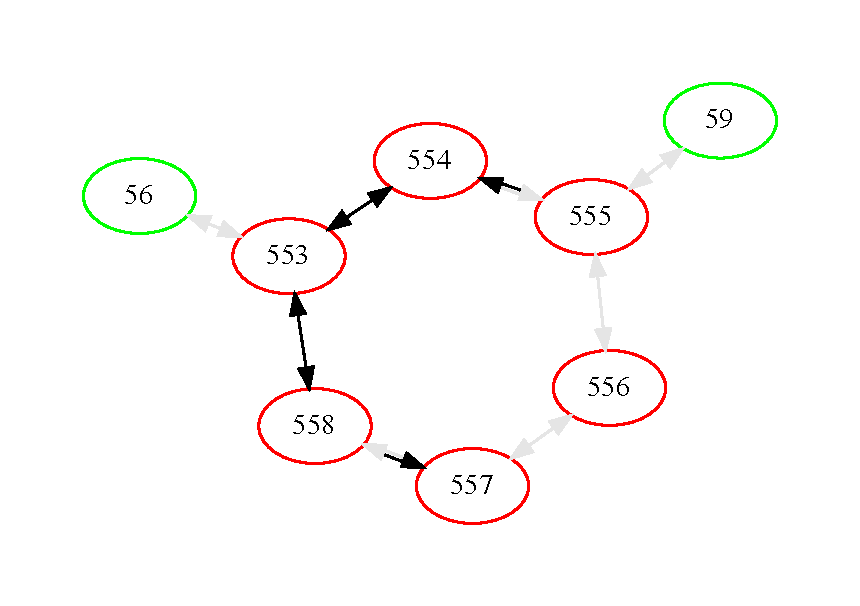
\includegraphics[width=0.95\linewidth]{images/tree-cycles-557.pdf}
	\end{subfigure}
	\begin{subfigure}{0.49\textwidth}
		\centering
		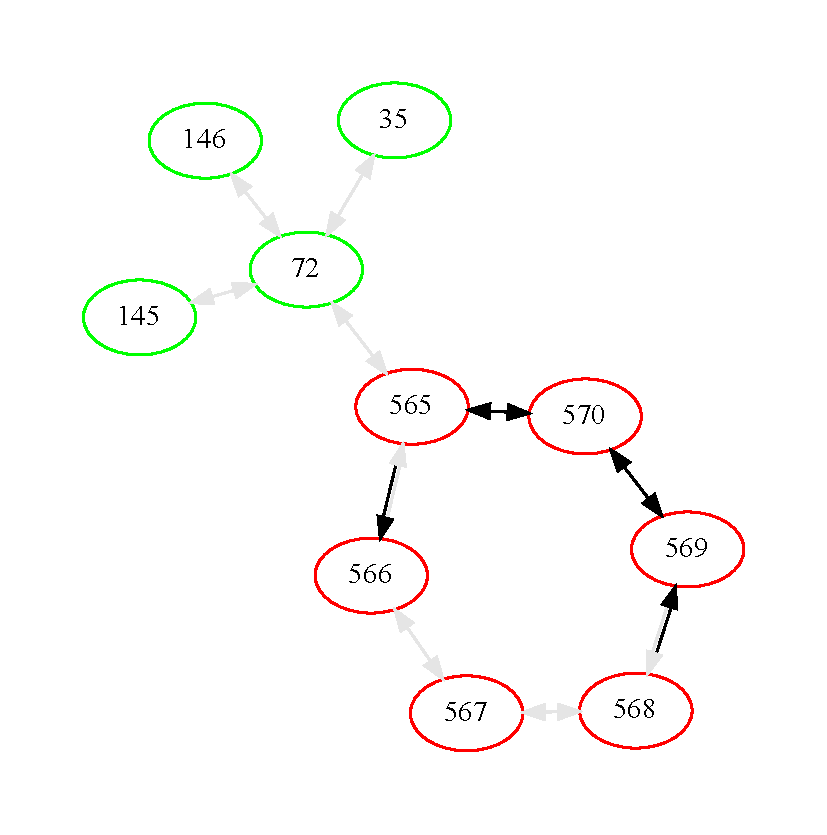
\includegraphics[width=0.95\linewidth]{images/tree-cycles-566.pdf}
	\end{subfigure}
	\begin{subfigure}{0.49\textwidth}
		\centering
		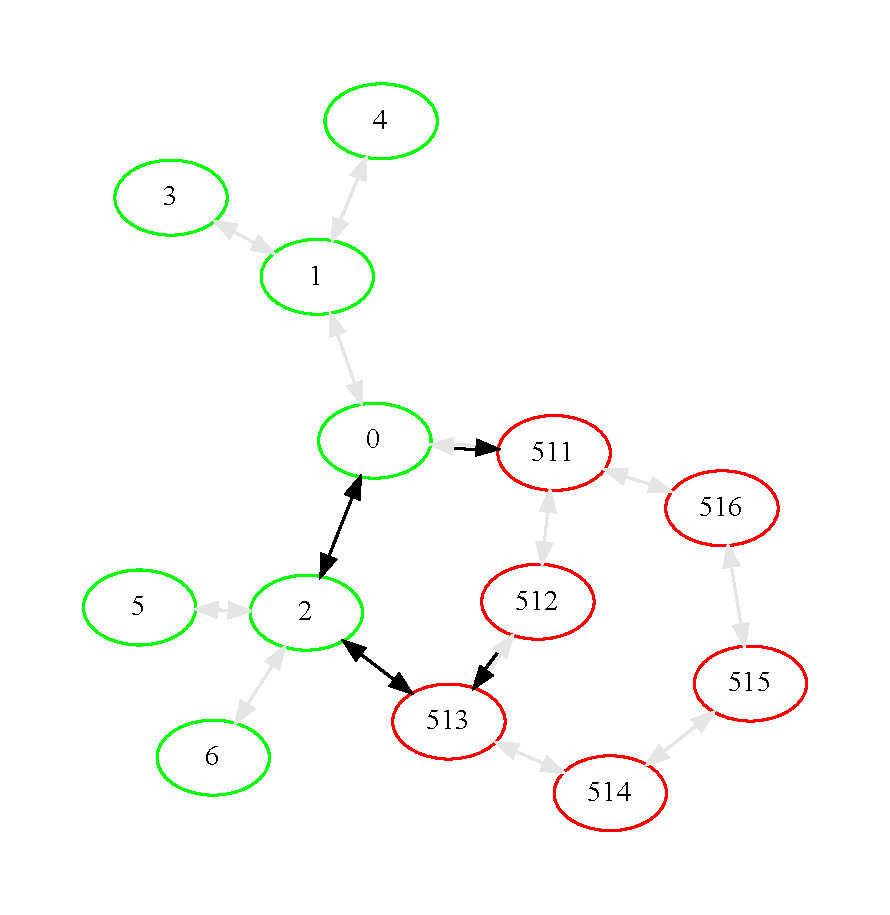
\includegraphics[width=0.95\linewidth]{images/tree-cycles-511.pdf}
	\end{subfigure}
	\caption{Found best subgraphs of size six for nodes 557, 566, and 511}
	\label{fig:tree-cycles-gt}
\end{figure}

Indeed, in none of the examples did a full ring structure get predicted. For nodes 557 and 566 it is clear that the most important subgraph uses about half the ring and has feedback structures inside of it with edges going both ways on intermediate nodes. In node 511, the interpretation barely comes from the ring structure and the GNN passes information through the edges of the tree structures. Clearly, it is not obvious that the motifs that the graph was defined on are not the groundtruth. Furthermore, the groundturth is \textit{highly} dependent on the GNN that is trained. With regards to the tree-cycle dataset, there are many different GNNs that peform equally well but have different groundtruths. Hence, it is difficult to use this dataset for GNN interpretation validation. While one could train GNNs until the motifs do become the correct groundtruth, it is hard to validate that any training run has achieved this goal.

One interesting thing to note here is that all three of these examples have the same structure i.e. a node points to an intermediate node that is fully connected (forwards and backwards) with the next node. This node fully connects to a third node before finally connecting to the target node. In this sense, the GNN has learned a general method for identifying cycles but it is not dependent on sending the information through solely cycle edges as seen by the ground truth for node 511.

\subsection{Noise Filtering Experiment}
While the tree-cycles dataset has its issues, it does serve as a good dataset to test GNNs on due to the fact that all of the performance in the model must be coming from the graph structure that is fed into the GNN. The node features contribute nothing and without any graph at all, the GNN will perform poorly. Hence, the first experiment proposed is a noise filtering experiment where we test the ability of GNN interpretation methods to detect and filter true negatives from their prediction of what is important to a model.

This is done by training a GNN on the tree-cycles dataset and then sampling noisy edges into the graph that did not exist previously. Then the GNN Interpretation methods are run on top of the noisy graph to see whether or not they will mistakenly choose noisy edges as important. Crucially, we do not care about what the groundtruth is but, rather, what it cannot possibly be. 

For adding the noise, inspiration is taken from \cite{dibaeinia_sergio_2020} and their addition of technical noise to single-cell expression data. Specifically, noise is added as described in listing \ref{alg:noise}.
\begin{algorithm}[h]
	\centering
	\caption{Sampling noise into tree-cycle dataset}
	\label{alg:noise}
	\begin{algorithmic}
		\Require $\lambda \geq 1$, $\rho \geq 2$.
		\State $\bar{E} \gets []$
		\For{$v \in V$}
			\State $n \sim Possion(\lambda)$
			\State $e \sim Categorical_n\left(\frac{1}{\sum_{v_i \in \mathcal{N}_{\rho}(v, E)}d(v, v_i)}[d(v, v_i) \mid \forall v_i \in \mathcal{N}_{\rho}(v, E)] \wedge d(v, v_i) \neq 1 \right)$
			\State $\bar{E} \gets \bar{E} \cup e$
		\EndFor
		\State $E \gets E \cup \bar{E}$
		\State $\mathcal{W}(e) \gets 1 \quad\quad \forall e \in E$
	\end{algorithmic}
\end{algorithm}
As a short summary, for each node $v$ in the graph a number of edges is sampled from $n \sim Possion(\lambda)$. This represents the amount of noisy edges that are going to be added going away from that node. Then, $n$ nodes are chosen at random from the $\rho$-hop neighborhood of $v$ with the probability of that noisy edge being added being defined as the inverse of the distance between the two nodes on the graph. Note, we restrict this to nodes that are more than distance one away. Once these noisy edges are sampled, they are added to a list that will all be added at once at the end of the sampling process. Note that in this case, we assume that the function $\mathcal{W}$ is always equal to one. With the right parameters $\lambda$ and $\rho$, we want to make sure the GNN performance does not degrade but we are adding in ample noise to the graph for the interpretation methods to filter out.

\subsubsection{Validation of GNN Performance}
To find the right parameters $\lambda$ and $\rho$, we need to ensure that the noise that is added is not too high but also that there is a significant challenge for the interpretation methods. The heatmap in figure \ref{fig:gnn-deg} shows the GNNs performance across a matrix of $\rho$ and $\lambda$ values.
\begin{figure}[h]
	\centering
	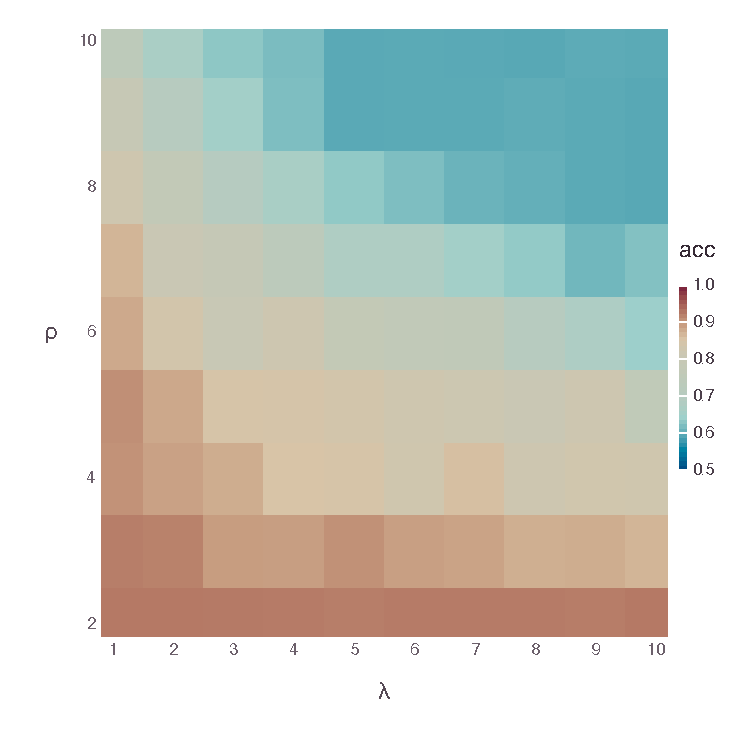
\includegraphics[width=0.75\textwidth]{images/gnn-noise-deg.pdf}
	\caption{Performance of the noisy tree-cycle experiment across a variety of $\lambda$ and $\rho$ values}
	\label{fig:gnn-deg}
\end{figure}

Note that before noise was added to the graph, all nodes had 2-4 connections in and out. As can be seen, the performance of the model is very good across almost all $\lambda$ values and $\rho$ values up to four. This indicates that the GNN is quite resiliant to noise and that GNN Interpretation methods should be able to filter out most of the noise if constructed correctly. In this case, we choose $\lambda = 2.5$ and $\rho = 3$ since this would give each node a rougly 50\% postitive to negative ratio on original edges to noisy edges. In this scheme, the GNN still performs well with roguhly 92\% accuracy.

\subsection{Graph Embedding Experiment}
For a more comprehensive test, we aim to create a GNN task in which the ground truth is known before-hand. From this we can generate a dataset where the GNN, provably, only utilizes the ground truth and nothing else. Note, that there is no way to ensure that the GNN utilizes each edge in the ground truth, but the aim is to ensure that a subset of the edges is used for each example in the dataset.

For this task, we define a graph classification task upon a complete graph of size seven. In this task, we define a Markov random walk over the nodes of the complete graph wherein a subset of the edges are biased. The level of bias is determined by a parameter $p$ that can be set at different values to generate different classes. Specifically, in figure \ref{fig:graph-bias-model}, one can see the embeded biased graph structure.
\begin{figure}[h]
	\centering
	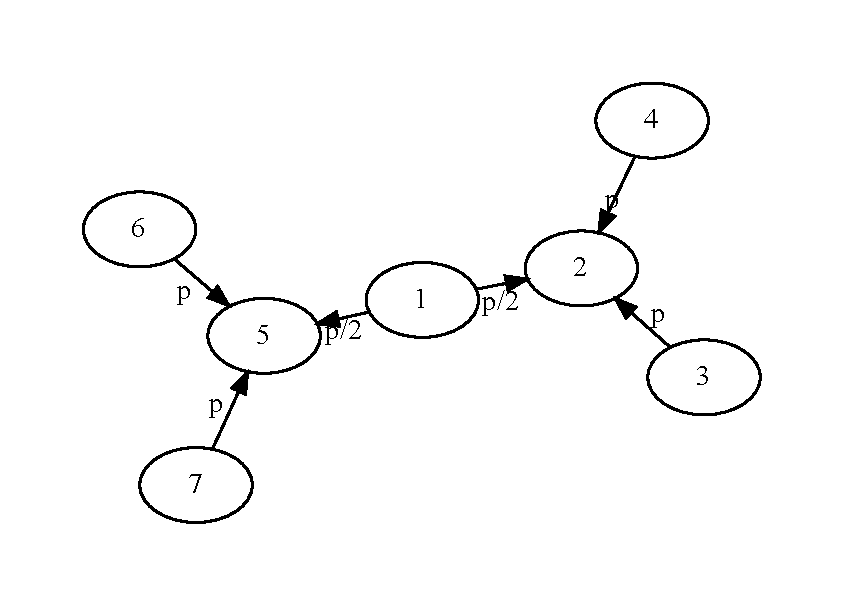
\includegraphics[width=0.9\textwidth]{images/tree-model.pdf}
	\caption{The biased portion of $K_7$ in the dataset generation. The rest of the edges are not drawn for clarity but have equal probability to each other node.}
	\label{fig:graph-bias-model}
\end{figure}
Other than the biased edges, all other edges have equal probability given as $\frac{1 - p}{5}$ except for node one which has all other edges having probability $\frac{1 - p}{4}$ (there are no self-edges). Hence, given this structure and a random walk over the nodes, the node feature for each node in the dataset is the number of times it is visited only if it is visited via an edge in the ground truth. In this way, the counts distribution is necessarily dependent on the ground-truth structure and a GNN will pick up on that.

\subsubsection{Dataset Details}
In particular, the dataset was generated with class label zero corresponding to $p = 0.4$ while class label one had $p = 0.675$. Additionally, each point in the dataset was generated by taking 75 hops on the random walk and the counts were then aggregated on a per-node basis. Finally, we had that each class had 500 samples each for a total of 1000 samples for the GNN to classify. The dataset also exhibits bimodal distributions for nodes 1, 2, and 5 with the overall distribution being best fit as a mixture of binomial distributions. In figure \ref{fig:tree-model-marginal-counts}, one can see the marginal counts distributions for each of nodes 1, 2, 5, and 6 (the rest of the nodes, by definition, cannot have any count). 
\begin{figure}[h]
	\centering
	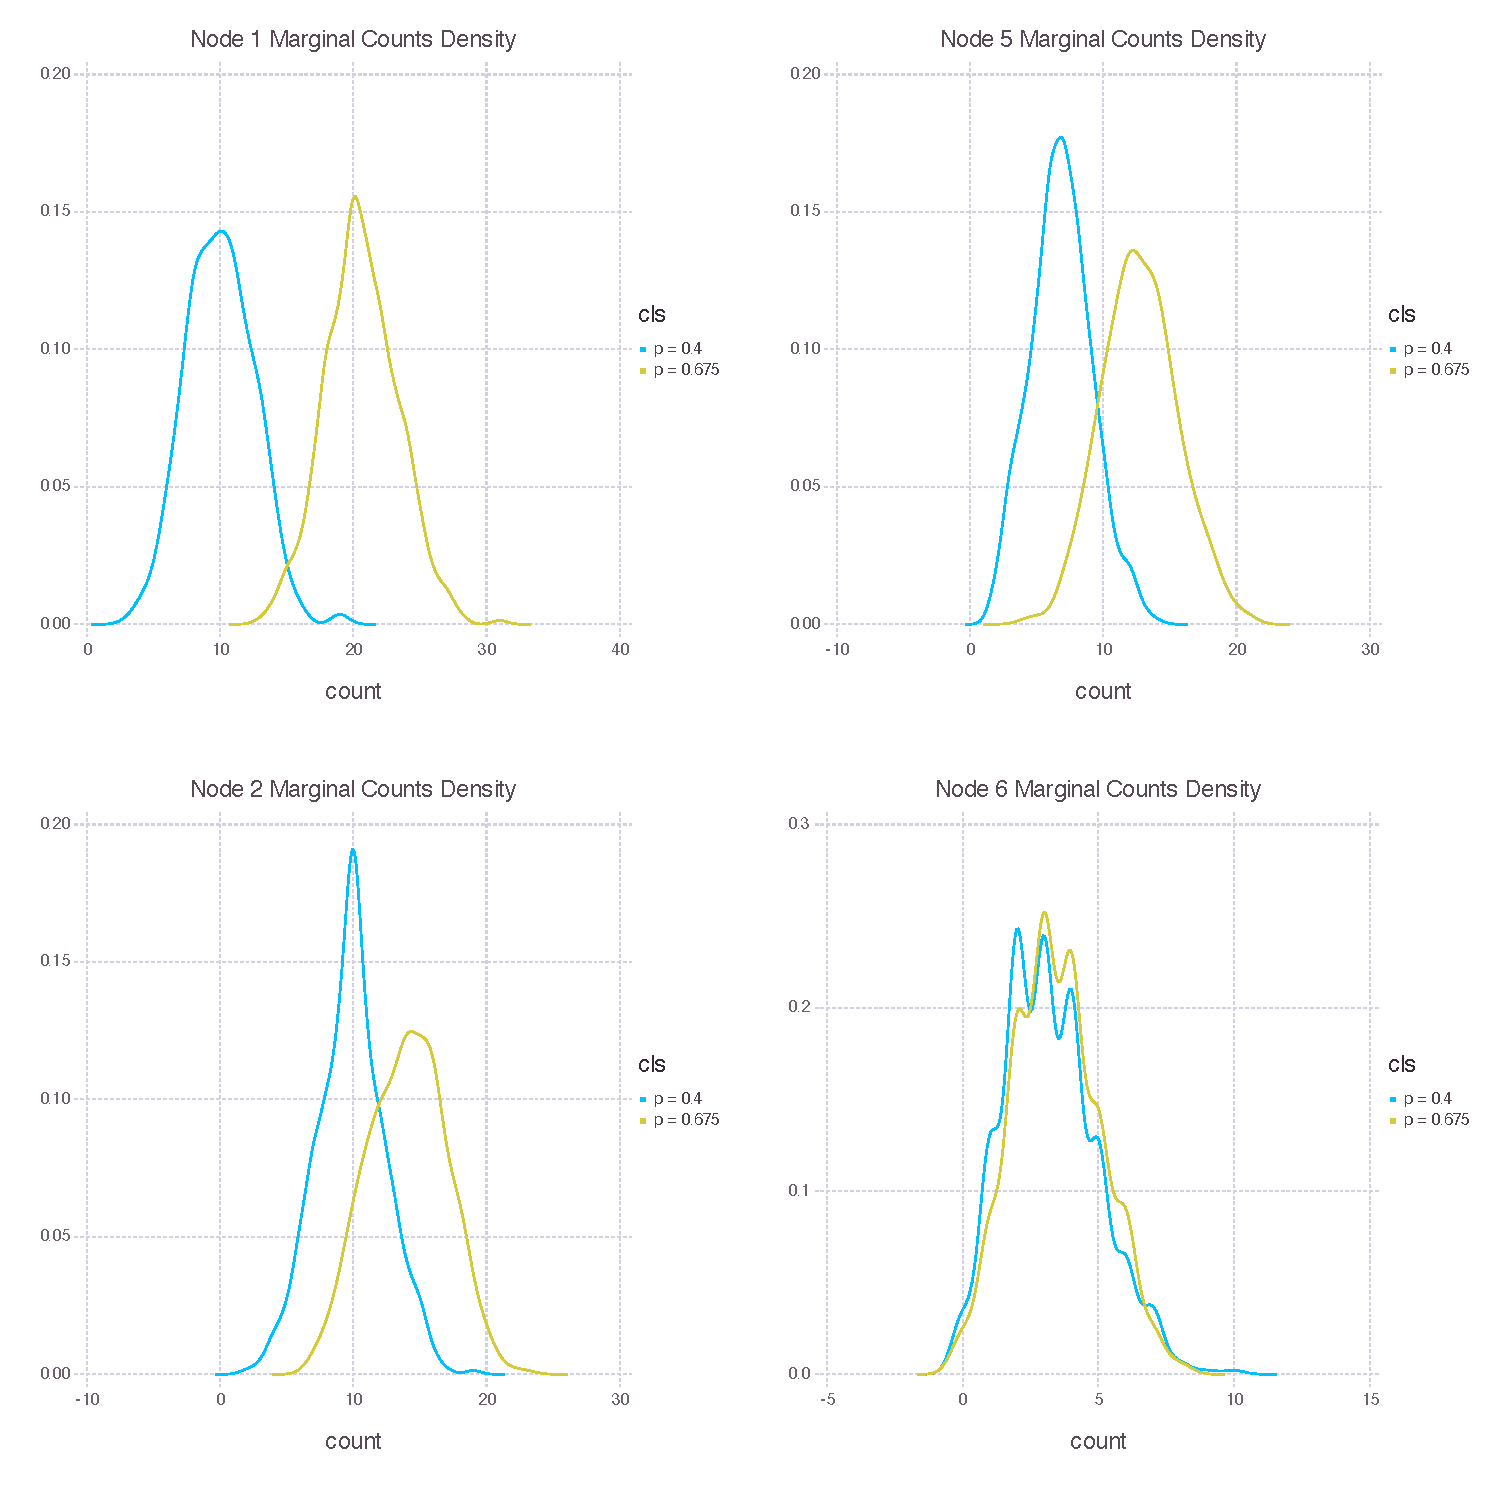
\includegraphics[width=0.8\textwidth]{images/tree-model-counts.pdf}
	\caption{Marginal counts distributions for each node with counts}
	\label{fig:tree-model-marginal-counts}
\end{figure}
Since node six, can only get counts from node seven, the two classes have very little differentiation on that node.

\subsubsection{GNN Performance Validation}
We know that if the counts values were not conditional on the groundtruth, the counts distribution overall would represent the steady-state distribution of the Markov process. In this case, each node distribution would be independent of each other and the optimal classifier would necessarily be a Naive Bayes multinomial classifier \cite{zhang_exploring_2005}. The groundtruth conditional distributions mean that the features are not independent which means that Naive Bayes is non-optimal. As a comparison, though, we trained a Naive Bayes classifier on this problem and got a test accuracy of 72.2\% showing that there is a lot of information to be gained by utilizing the graph structure.  

Indeed, we trained the GNN on this problem by feeding it the entire computational graph, but validated its accuracy on fresh examples and the entire groundtruth graph getting an accuracy of 99\%. Hence, there is strong reason to believe that the GNN learned from the graph groundtruth. To validate this even further, we checked a few metrics with the trained GNN. First the accuracy of the GNN was measured when the entire computational graph was fed in, with the strength of the edges going from 0 to 1 in 0.1 increments. The same was repeated with the groundtruth and the inverse of the groundtruth (all of the noisy edges). In figure \ref{fig:tree-model-sparsity}, the results of this experimentation can be seen. 
\begin{figure}[h]
	\centering
	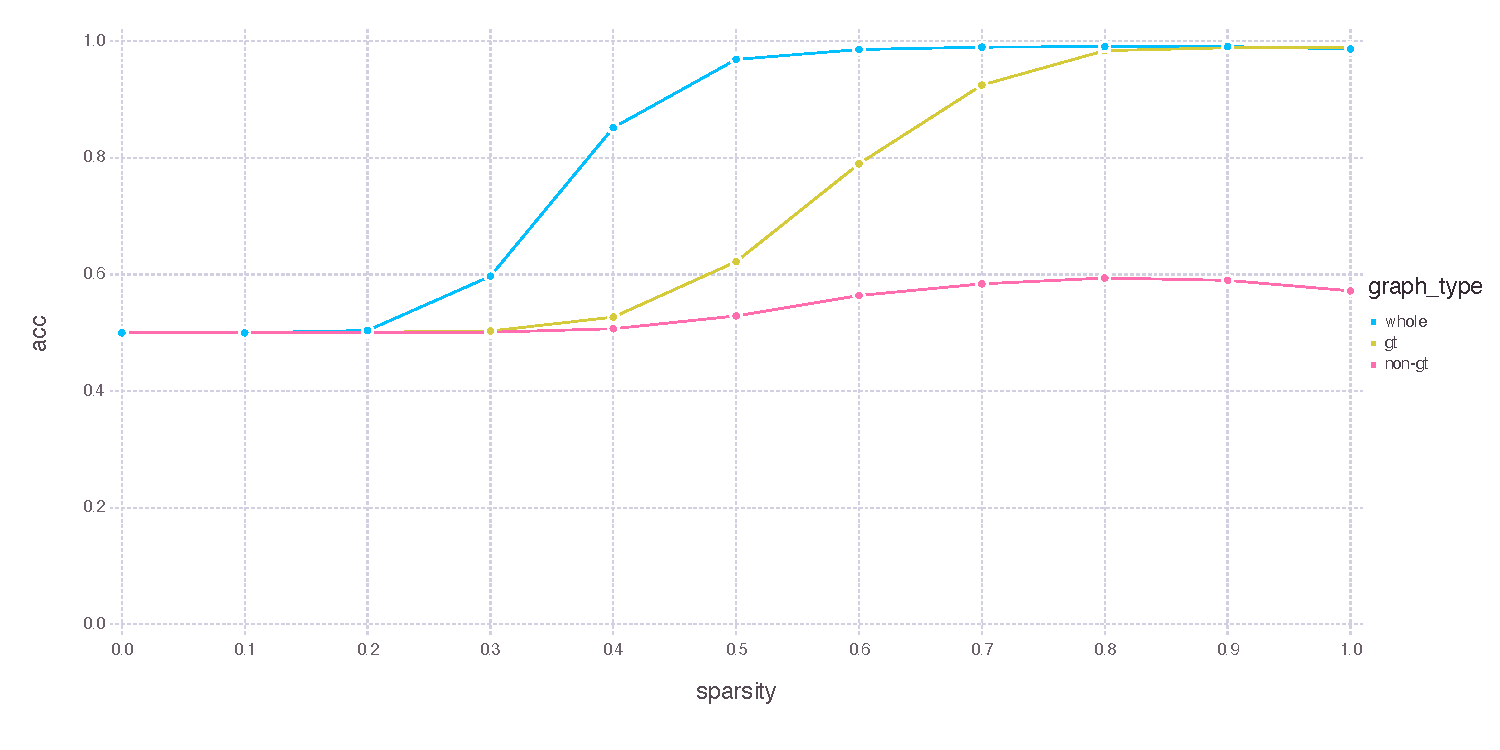
\includegraphics[width=0.9\textwidth]{images/tree-model-sparsity.pdf}
	\caption{Performance of the GNN at different sparsity with (a) the entire computational graph (b) the groundtruth and (c) the inverse of the groundtruth}
	\label{fig:tree-model-sparsity}
\end{figure}

While the performance of the whole computational graph increases faster than that of the groundtruth, they ended up with the same accuracy at level 0.8 and it is clear that the inverse of the groundtruth contains very little information as its performance improved very little. What this indicates is that the groundtruth is very essential to the performance of the GNN and that a subset of it for any given node is essential for the predictive power of the GNN. Note that because for class zero the GNN automatically predicts the correct answer, only class one examples are used for the actual interpretation challenge. Hence, this seems like a strong candidate for evaluating GNN interpretation performance. While not all edges in the groundtruth may be needed for each example, all explainer tasks will be at the same disadvantage meaning that the results will be comprable.

\newpage
